% \chapter{RGB-D SLAM}\label{rgbd-slam}

% Range sensors have emerged as one of the most effective sensors to make robots autonomous. Unlike vision, range data makes the construction of a 3D model of the robot's environment straightforward and the Velodyne sensor, that combines 64 scanning lasers into one package, was key in mastering the DARPA Grand Challenge.  3D range data has become even more important in robotics with the advent of cheap (priced at a tenth than the cheapest 2D laser scanner) RGB-D (color image plus depth) cameras. Point cloud data allows fitting of lines using RANSAC, which can serve as features in EKF-based localization, but can also be used for improving odometry, loop-closure detection, and mapping. The goals of this chapter are

\chapter{RGB-D SLAM} 
\label{rgbd-slam}

距离传感器已成为使机器人实现自主的最有效的传感器之一。与视觉不同,距离数据使得机器人环境的三维模型的构建简单直观,Velodyne传感器将64个扫描激光器封装到一起,是在DARPA大挑战(DARPA Grand Challenge)中获胜的关键。随着近来价格便宜(比二维激光扫描仪便宜十分之一)的RGB-D相机(彩色图像加深度)出现,三维距离数据变得更加重要。点云数据使我们可以使用RANSAC拟合直线,其可以作为基于扩张卡尔曼滤波(EKF)定位的特征,但也可用于改进里程计、闭环检测和建图。本章的目标是

\begin{itemize}
% \item introduce the Iterative Closest Point (ICP) algorithm
% \item show how ICP can be improved by providing initial guesses via RANSAC
% \item show how SIFT features can be used to improve point selection and loop-closure in ICP to achieve RGB-D mapping

\item 介绍迭代最近点(ICP)算法
\item 介绍如何通过RANSAC提供初始估计来改进ICP
\item 介绍如何用SIFT特征改进ICP中的点选择和闭环,以实现RGB-D建图
\end{itemize}

% \section{Converting range data into point cloud data}
% Point cloud data can be thought of a 3D matrix that maps a certain volume in 3D space. Each cell in this matrix, also known as \emph{Voxel}\index{Voxel}, corresponds to whether there is an obstacle in this volume or not. Different intensity values could correspond to the uncertainty with which this space is to be known to be an obstacle. An efficient method to turn range information into such an uncertainty 3D map is described in \cite{curless96} and became known as \emph{Truncated Surface Distance Function} (TSDF)\index{Truncated Surface Distance Function (TSDF)}\index{TSDF}, commonly referred to as ``Point cloud''\index{Point cloud}.

\section{将距离数据转换为点云数据}
点云数据可以被认为是在三维空间中映射某个体积的三维矩阵。该矩阵中的每个单元格,也称为\emph{Voxel}\index{Voxel},对应于此体积中是否存在障碍物。不同的强度值可以表示该空间有障碍物的不确定性/概率。在\cite{curless96}中描述了将距离信息转换为这种不确定性三维映射的有效方法,并被称为\emph{截断表面距离函数}(Truncated Surface Distance Function,TSDF)\index{截断表面距离函数(Truncated Surface Distance Function,TSDF)}\index{TSDF},通常称为“点云”\index{点云(Point cloud)}。

% \section{The Iterative Closest Point (ICP) algorithm}
% The \emph{Iterative Closest Point} (ICP)\index{Iterative Closest Point}\index{ICP} algorithm was presented in the early 1990s for registration of 3D range data to CAD models of objects. A more in-depth overview of what is described here is given in \cite{rusinkiewicz01}. The key problem can be reduced to find the best transformation that minimizes the distance between two point clouds. This is the case when matching snapshots from a range sensor or matching a range image with a point cloud sampled from a 3D representation of an object.

\section {迭代最近点(ICP)算法}
20世纪90年代初,\emph{迭代最近点(Iterative Closest Point,ICP)}\index{迭代最近点(Iterative Closest Point,ICP)}\index{ICP}算法被提出,用于将三维距离数据对应到CAD的物体模型。在\cite{rusinkiewicz01}中给出了更详细的概述。关键问题可以被简化为找到最小化两点云之间距离的最佳变换。将距离传感器快照或者距离图像与从物体的三维表示中采样的点云匹配,就是这种思路。

% In robotics, ICP found an application to match scans from 2D laser range scanners. For example, the transformation that minimizes the error between two consecutive snapshots of the environment is proportional to the motion of the robot. This is a hard problem as it is unclear, which points in the two consecutive snapshots are ``pairs", which of the points are outliers (due to noisy sensors), and which points need to be discarded as not all points overlap in both snapshots. Stitching a series of snapshots together theoretically allows to create a 2D map of the environment. This is difficult, however, as the error between every snapshots --- similar to odometry --- accumulates.   The ICP algorithm also works in 3D where it allows to infer the change in 6D pose of a camera and creation of 3D maps. In addition, ICP has proven useful for identifying objects from a database of 3D objects.

在机器人技术方面,ICP被发现可以用来匹配二维激光距离扫描仪的扫描图。例如,最小化两个连续的环境快照之间的误差的变换与机器人的运动成比例。这是一个困难的问题,因为它不清楚连续两个快照中的哪些点是“对应的”,哪些点是异常点(由于噪声传感器),哪些点需要丢弃,因为并不是所有点都出现在两张快照中。理论上,将的一系列快照拼接在一起可以创建环境的二维地图,但这是困难的,因为每个快照之间的误差会累积(类似于里程计),ICP算法也可以用在三维中,它可以推断出摄像机的六维姿态的变化和创建三维地图。此外,ICP已被证明从三维物体的数据库中识别物体很有效。

% Before providing a solution to the mapping problem, we will focus on the ICP algorithm to match 2 consecutive frames. Variants of the ICP algorithm can be broken down into 6 consecutive steps:

在提供建图问题的解决方案之前,我们将重点关注ICP算法来匹配2个连续帧。 ICP算法的变种可以分为6个步骤:

\begin{enumerate}
% \item Selection of points in one or both meshes or point clouds.
% \item Matching/Pairing these points to samples in the other point cloud/mesh.
% \item Weighting the corresponding pairs.
% \item Rejecting certain pairs.
% \item Assigning an error metric based on the point pairs.
% \item Minimizing the error metric.
% \item Point Selection

\item 选择在一个或两个网格或点云中的点。
\item 将这些点与另一个点云/网格中的采样点进行匹配/配对。
\item 评估这些点对。
\item 抛弃某些点对。
\item 根据分配点对误差度量。
\item 最小化误差度量。
%\item 选择点
\end{enumerate}

% Depending on the number of points generated by the range sensor, it might make sense to use only a few selected points to calculate the optimal transformation between two point clouds, and then test this transformation on all points. Depending on the source of the data, it also turns out that some points are more suitable than others as it is easier to identify matches for them. This is the case for RGB-D data, where SIFT features have been used successfully. This is also the case for planar objects with grooves, where sampling should ensure that angles of normal vectors of sampling points are broadly distributed. Which method to use is therefore strongly dependent on the kind of data being used and should be considered for each specific problem.

根据距离传感器产生的点数,只使用一些选定的点来计算两个点云之间的最佳变换,然后在所有点上测试此转换,这可能是有意义的。根据数据的来源,一些点比其他点更合适,因为更容易识别它们的匹配。这适用于RGB-D数据,其中SIFT特征已成功使用。对于有槽的平面物体也是如此,其中采样时应确保采样点的法向量的角度广泛分布。因此,使用哪种方法很大程度上取决于所使用的数据类型,应针对每个具体问题进行考虑。

% \subsection{Matching Points}
% The key step in ICP is to match one point to its corresponding point.  For example, a laser scanner hits a certain point at a wall with its 67th ray. After the scanner has been moved by 10 cm, the closest hit on the wall to this point might have been by the 3rth ray of the laser. Here, it is actually very unlikely that the laser hits the exact same point on the wall twice, therefore introducing a non-zero error even for optimal pairing. Prominent methods are to find the closest point in the other point cloud or to find the intersection of the source points normal with the destination surface (for matching point clouds to meshes). More recently, SIFT has allowed to match points based on their visual appearance. Similarly to sorting through SIFT features, finding the closest matching point can be accelerated by representing the point cloud in a k-d tree.

\subsection{匹配点}
ICP的关键步骤是将一点与其对应点相匹配。例如,激光扫描仪的第67号射线击中墙上的某一点。在扫描仪移动了10厘米后,墙上最接近的这一点的点可能是激光的第3条光线击中的。在这里,激光器实际上不太可能两次击中墙上完全相同的点,因此即使是最佳匹配也要引入非零误差。著名的方法是找到另一个点云中的最近点,或者找到源点与目标表面(用于把点云匹配到网格上)正交的交点。最近,SIFT已经可以基于它们的视觉外观来匹配点。类似于根据SIFT特征排序,把点云表示为k-d树可以加快找到最接近的匹配点。

% \subsection{Weighting of Pairs}
% As some pairs are better matches than others, weighting them in some smart way might drastically improve the quality of the resulting transformation. One approach is to give more weight to points that have smaller distances from each other. Another approach is to take into account the color of the point (in RGB-D images) or use the distance of their SIFT features (weighting pairs with low distances higher than pairs with high distances). Finally, expected noise can be used to weight pairings. For example, the estimates made by a laser scanner are much more faithful when taken orthogonally to a plane than when taken at a steep angle.

\subsection {点对的权重}
由于某些点对比其他点对匹配度更好,因此以一些聪明的方式对它们进行加权可能会大大提高得到变换的质量。一种方法是对相互距离较小的点给予更大的权重。另一种方法是考虑到点(RGB-D图像)的颜色,或者使用它们的SIFT特征的距离(距离近的点对权重比距离远的点对权重大)。最后,期望噪声可以用于评估点对。例如,与以陡峭的角度拍摄相比,以与平面正交的角度拍摄,激光扫描仪的估计值更加可靠。

% \subsection{Rejecting of Pairs}
% A key problem in ICP are outliers either from sensor noise or simply from incomplete overlap between two consecutive range images. A prime approach in dealing with this problem is to reject pairings of which one of the points lies on a boundary of the point cloud as these points are likely to match with points in non-overlapping regions. As a function of the underlying data, it might also make sense to reject pairings with too high of a distance. This is a threshold-based equivalent to distance-based weighting as described above.

\subsection{抛弃点对}
ICP的一个关键问题是来自传感器的噪声或简单的来自两个连续距离图像之间的不完全重叠。处理这个问题的一个主要方法是抛弃哪些其中一点位于点云边界上的点对,因为这些点可能与非重叠区域中的某点相匹配。作为潜在数据的功能,抛弃距离太远的点对也可能会有用。这种基于阈值的方法,等价于上文中基于距离的权重法。

% \subsection{Error Metric and Minimization Algorithm}
% After points have been selected and matched, pairs have been weighted and rejected, the match between two point clouds needs to be expressed by a suitable error metric, which needs then to be minimized. A straightforward approach is to consider the sum of squared distances between each pair. This formulation can often be solved analytically. Let

\subsection{误差度量和最小化算法}
在选择并匹配点对之后,点对已经被赋予权重和删减,两个点云之间的匹配需要由适当的误差度量来表示,然后需要将其最小化。一个简单的方法是考虑每个点对之间距离的平方和。这个表达式通常可以用解析法求解。 令

\begin{eqnarray}
A=\{a_1,\ldots,a_n\}\\
B=\{b_1,\dots,b_n\}
\end{eqnarray}

% be point clouds in $ \mathbb{R}^n$. The goal is now to find a vector $ t \in \mathbb{R}^n$ so that an error function $ \phi(A+t,B)$ is minimized. In 6D (translation and rotation), an equivalent notation can be found for a transformation (see forward kinematics). An error function for the squared distance is then given by

为$\mathbb{R}^n$中的点云。目标是找到一个向量$t\in\mathbb{R}^n$,以使误差函数$\phi(A+t,B)$最小。在六维(平移和旋转)中,可以找到一个变换的等效符号(见正运动学)。然后距离平方的误差函数为

\begin{equation}
\phi(A+t,B)=\frac{1}{n}\sum_{a \in A}\|a+t-N_B(a+t)\|^2
\end{equation}

% Here $ N_B(a+t)$ is a function that provides the nearest neighbor of $ a$ translated by $ b$ in $ B$.  A key problem now is that the actual value of $t$ affects the outcome of the pairing. What might look like a good match initially often turns out not be the final pairing. A simple numerical approach to this problem is to find $ t$ iteratively.

其中$N_B(a+t)$是一个函数,它表示由$B$中$b$平移的$a$的最近邻。现在的关键问题是$t$的实际值影响匹配的结果。最初看起来合适的匹配,往往不是最终匹配。这个问题的一个简单的数值方法是迭代地找到$t$。

% Initially $t=0$ and nearest neighbors/pairings are established. We can now calculate a $ \delta t$ that optimizes the least-square problem based on this matching using any solver available for the optimization problem (for a least-square solution $ \delta t$ can be obtained analytically by solving for the minimum of the polynomial by setting its derivative to zero). We can then shift all points in $ A$ by $ \delta t$ and start over. That is, we calculate new pairings and derive a new $ \delta t$.  We can continue to do this, until the cost function reaches a local minimum.

最初$t=0$,建立最近邻/匹配。现在我们可以计算最优化基于这种匹配的最小二乘问题的$\delta t$,可以利用求解优化问题的任何求解器(对于最小二乘解决方案,$\delta t$可以通过解析求多项式最小化来获得,即将其导数设置为零)。然后我们可以将$A$中的所有点平移$\delta t$并重新开始。也就是说,我们计算新的匹配并推导出一个新的$\delta t$。我们可以继续这样做,直到成本函数达到局部最小值。

% Instead of formulating the cost function as a ``point-to-point'' distance, a ``point-to-plane'' has become popular. Here, the cost function consist of the sum of squared distances from each source point to the plane that contains the destination point and is oriented perpendicular to the destination normal. This makes particularly sense when matching a point cloud to a mesh/CAD model of an object. In this case there are no analytical solutions to finding the optimal transformation, but any optimization method such a Levenberg-Marquardt can be used.

用“点到平面”,而不是“点到点”的距离定义成本函数变得流行起来。这里,成本函数为每个源点到平面的距离平方和,这个平面包含目标点,并垂直于目标法线。当将点云匹配到物体的网格/CAD模型时,这是特别有意义的。在这种情况下,没有获得最佳变换的解析求解方案,但是可以使用诸如Levenberg-Marquardt之类的任何优化方法。

% \section{RGB-D Mapping}
% The ICP algorithm can be used to stitch consecutive range images together to create a 3D map of the environment \cite{henry2010rgb}. Together with RGB information, it is possible to create complete 3D walk throughs of an environment. An example of such a walk through using the method described in \cite{whelan2013robust} is shown in Figure \ref{fig:kintinous}.

\section{RGB-D建图}
ICP算法可用于将连续距离图像拼接在一起,以创建环境的三维地图\cite{henry2010rgb}。与RGB信息一起,可以创建环境完整的3D漫游。使用\cite{whelan2013robust}中描述的方法进行的这种漫游的例子如图\ref{fig:kintinous}所示。

% A problem with ICP is that errors in each transformation propagate making maps created using this method as odd as maps created by simple odometry. Here, the SLAM algorithm can be used to correct previous errors once a loop closure is detected.

ICP的一个问题是,每个变换中的误差传播,使得用这种方法创建的地图与由简单里程计创建的地图一样奇怪。这里,一旦检测到环路闭合,SLAM算法就可用于校正以前的误差。

\begin{figure}
\centering
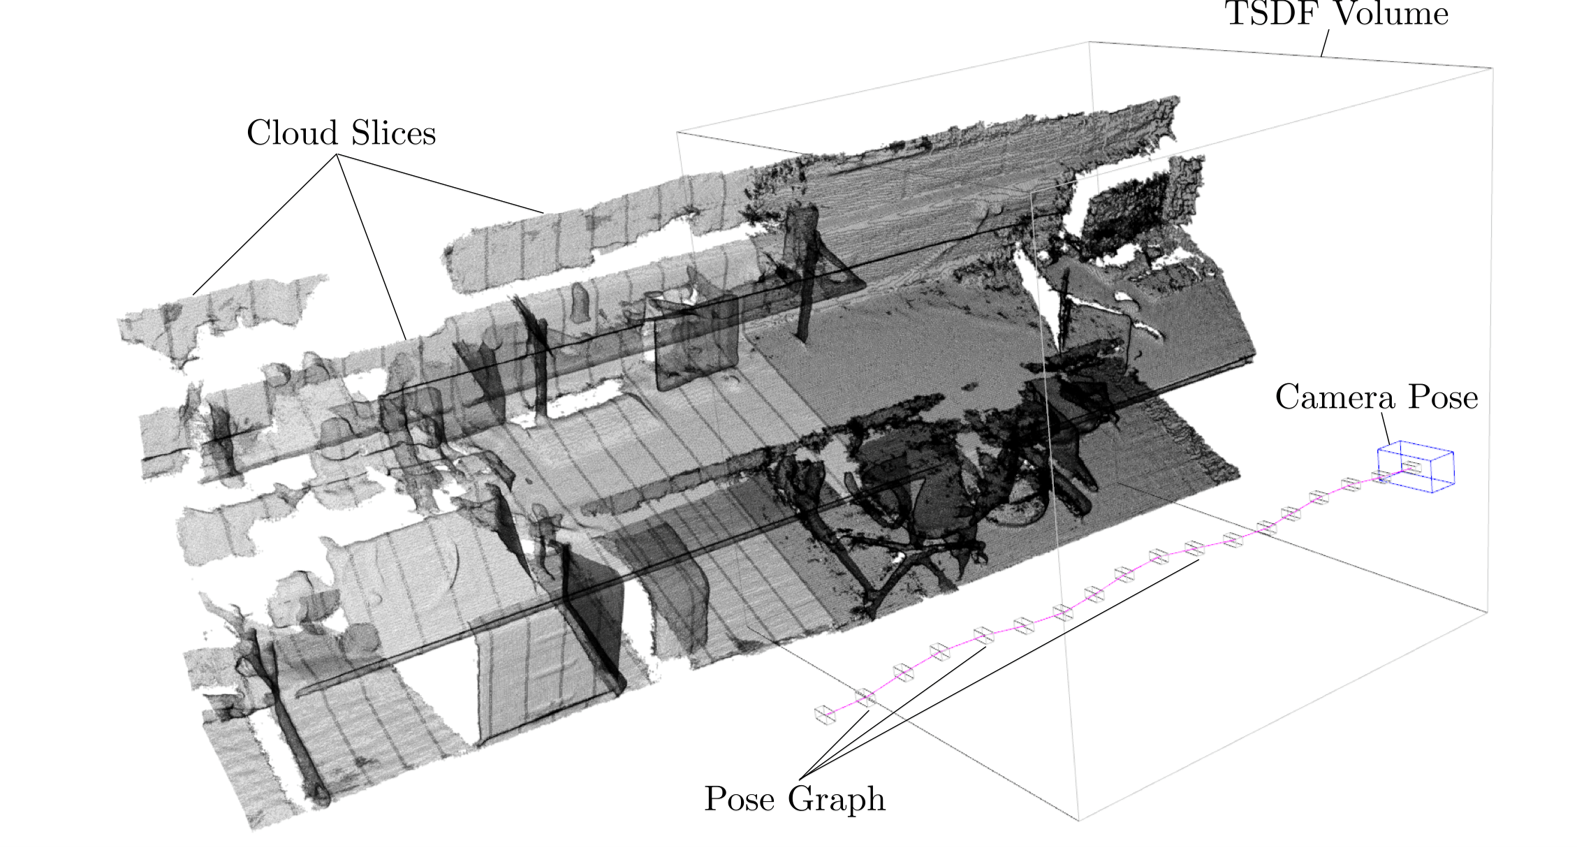
\includegraphics[width=\textwidth]{figs/kintinous}
% \caption{Fused point cloud data from a walk trough of an office environment using ``Kintinious''. Picture courtesy of John Leonard.}
\caption{使用“Kintinious”的办公环境漫游的融合点云数据。图片由约翰·伦纳德(John Leonard)提供。}
\label{fig:kintinous}
\end{figure}

% The intuition behind SLAM is to consider each transformation between consecutive snapshots as a spring with variable stiffness. Whenever the robot returns to a previously seen location, i.e., a loop-closure has been determined, additional constraints are introduced and the collection of snapshots connected by springs become a mesh. Everytime the robot then re-observes a transformation between any of the snapshots, it can ``stiffen'' the spring connecting the two. As all of the snapshots are connected, this new constraints propagates through the network and literally pull each snapshots in place.

SLAM背后的直观理解是将连续快照之间的每个变换视为具有可变刚度的弹簧。每当机器人返回到先前看到的位置时,即发现闭环,则引入额外的约束,并且弹簧连接的快照的集合变成网格。每当机器人再次观测到任何快照之间的变换时,它可以“强化”连接两个快照的弹簧。由于所有的快照都是连接的,所以新的约束通过网络传播,并逐步地将每个快照拉到位。

% RGB-D Mapping uses a variant of ICP that is enhanced by SIFT features for point selection and matching. Maps are build incrementally. SIFT features, and their spatial relationship, are used for detecting loop closures. Once a loop closure is detected, an additional constraint is added to the pose graph and a SLAM-like optimization algorithm corrects the pose of all previous observations.

RGB-D建图使用由用于选择和匹配点的SIFT特征增强的ICP的变种。地图逐步建立。SIFT特征及其空间关系用于检测闭环。一旦检测到闭环,一个额外的约束被添加到姿态图中,并且类SLAM优化算法校正所有先前观测到的姿态。

% As ICP only works when both point clouds are already closely aligned, which might not be the case for a fast moving robot with a relatively noisy sensor (the XBox Kinect has an error of 3cm for a few meters of range vs. millimeters in laser range scanners), RGB-D Mapping uses RANSAC to find an initial transformation. Here, RANSAC works as for line fitting: it keeps guessing possible transformations for 3 pairs of SIFT feature points and then counts the number of inliers when matching the two point clouds, one of which being transformed using the random guess.

由于ICP仅在两个点云已经紧密对齐的情况下才起作用,对于有一定噪声的传感器的快速移动机器人而言,这可能不是适用(XBox Kinect在几米距离内的误差为3厘米,而激光距离扫描仪为毫米级别)。RGB-D建图使用RANSAC来找到初始变换。这里,RANSAC适用于直线拟合:它持续猜测3对SIFT特征点的可能变换,然后计数匹配两个点云时的正常值数量,其中一个点云使用随机猜测进行变换。